\documentclass[12pt,letterpaper]{exam}
\usepackage[lmargin=1in,rmargin=1in,tmargin=1in,bmargin=1in]{geometry}
\usepackage{../style/exams}

% -------------------
% Course & Exam Information
% -------------------
\newcommand{\course}{MATH 115: Exam 3}
\newcommand{\term}{Fall --- 2024}
\newcommand{\examdate}{11/21/2024}
\newcommand{\timelimit}{50 Minutes}

\setbool{hideans}{true} % Student: True; Instructor: False


% -------------------
% Content
% -------------------
\begin{document}

\examtitle
\instructions{Write your name on the appropriate line on the exam cover sheet. This exam contains \numpages\ pages (including this cover page) and \numquestions\ questions. Check that you have every page of the exam. Answer the questions in the spaces provided on the question sheets. Be sure to answer every part of each question and show all your work. If you run out of room for an answer, continue on the back of the page --- being sure to indicate the problem number.} 
\scores
\bottomline
\newpage


% -------------------
% Questions
% -------------------
\begin{questions}

% Question 1
\newpage
\question[15] Compute the exact value for the following: \par\vspace{0.3cm}
	\begin{enumerate}[(a)]
	\item $\sin(240^\circ)=$ \vfill
	\item $\csc \!\left( \dfrac{2\pi}{3} \right)=$ \vfill
	\item $\tan \!\left(\dfrac{3 \pi}{2} \right)=$ \vfill
	\item $\sec(135^\circ)=$ \vfill
	\item $\cos(\pi)=$ \vfill
	\end{enumerate}



% Question 2
\newpage
\question[15] Compute the exact value for the following: \par\vspace{0.3cm}
	\begin{enumerate}[(a)]
	\item $\sin^{-1} \!\!\left( -\dfrac{1}{2} \right)=$ \vfill
	\item $\arccos \!\left( \dfrac{1}{\sqrt{2}} \right)=$ \vfill
	\item $\tan^{-1}(-1)$ \vfill
	\item $\arccos \!\left( \dfrac{\sqrt{3}}{2} \right)=$ \vfill
	\item $\arctan(-\infty)=$ \vfill
	\end{enumerate}



% Question 3
\newpage
\question[10] For each part below, give a trigonometric identity as described in the problem statement.
	\begin{enumerate}[(a)]
	\item Write $\cos(2x)$ in terms of \textit{both} $\sin(x)$ and $\cos(x)$. \vfill
	\item Write $\tan^2(x)$ in terms of \textit{only} $\sec(x)$. \vfill
	\item Write an identity for $\tan(A \pm B)$. \vfill
	\item Write an identity for $\sin(A \pm B)$. \vfill
	\end{enumerate}



% Question 4
\newpage
\question[20] Showing all your work, answer the following problems: \par\vspace{0.1cm}
	\begin{enumerate}[(a)]
	\item Compute $\sin \!\big( \!\arctan(-4) \big)$ \vfill
	\item If $\tan \theta= -\frac{5}{12}$ and $\cos \theta > 0$, compute $\sin(2 \theta)$. \vfill
	\end{enumerate}



% Question 5
\newpage
\question[10] Using the fact that $\dfrac{17\pi}{12}= \dfrac{5\pi}{3} - \dfrac{\pi}{4}$ and showing all your work, compute $\cos \left( \dfrac{17\pi}{12} \right)$. 



% Question 6
\newpage
\question[15] Find the value of $x$ in the triangle shown below. Be sure to show all your work.
	\[
	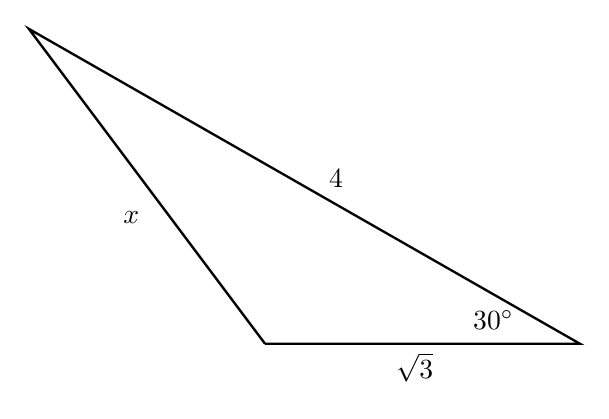
\begin{tikzpicture}
	\draw[line width=0.03cm] (0,0) -- (-3,4) -- (4,0) -- (0,0);
	\node at (-1.7,1.6) {$x$};
	\node at (1.9,-0.3) {$\sqrt{3}$};
	\node at (0.9,2.1) {$4$};
	\node at (2.9,0.3) {$30^\circ$};
	\end{tikzpicture}
	\]



% Question 7
\newpage
\question[15] Showing all your work, find all the exact solutions to the equation shown below. 
	\[
	8 \sin^2(2 \pi x - \pi) + 5= 9
	\]

\end{questions}
\end{document}